\documentclass[10pt, oneside]{article}   	
\usepackage[top=1in, bottom=1.25in, left=1in, right=1in]{geometry}     
\usepackage{float}		
\geometry{letterpaper}
\usepackage{fancyhdr}
\usepackage{hyperref}
\usepackage{enumerate}
\pagestyle{fancy}
\headheight 35pt 
\lhead{\sc Computer Science 181 \footnotesize{(Spring 2015)}}
\chead{}
\rhead{\sc George Wu, Lisa Wang, Allen Chen}
\rfoot{}
\cfoot{\thepage}
\lfoot{}                   		
\usepackage{graphicx}				
\usepackage{amsthm,amsmath,amssymb}
\newtheorem{question}{Question}
\newcommand\independent{\protect\mathpalette{\protect\independenT}{\perp}}
\def\independenT#1#2{\mathrel{\rlap{$#1#2$}\mkern2mu{#1#2}}}
%\usepackage{minted}
%\date{}							% Activate to display a given date or no date
\begin{document}
\centerline{\Large{\textbf{Practical 4: Reinforcement Learning}}}
\vspace{6px}
\section{Introduction}
In this practical, we try to learn the optimal policy for the monkey in the game Swingy Monkey. We'll adopt a reinforcement learning approach, using Q-Learning to try to learn the optimal actions at each state.
\section{State Space}
We tried several things to determine the optimal state space for reinforcement learning. First, we note that the set of possible positions in the space is very large, such that it was necessary to discretize the space into larger blocks rather than using individual spaces. Second, the state at any given time includes the distance to the next tree trunk, the screen height of the top of the tree trunk gap, the screen height of the bottom of the tree trunk gap, the velocity of the monkey, the screen eight of the top of the monkey, and the screen height of the bottom of the monkey. Using the absolute pixel height of both the monkey's top and bottom and tree's top and bottom would result in something along the magnitude of $600^4$ states, which would be far too many to use for Q-learning.  \\\\
The first configuration we tried was a tuple consisting of the difference between the height of the top of the monkey and the height of the top of the tree trunk gap, and the distance to the nearest tree. However, we were unable to achieve a score of more than 10-15 after 100 iterations. We observed that most of the deaths were being caused, not by running into a tree, but by falling off the screen, and thus altered our state configuration to take this into account. By observing the monkey's death behavior, we ended up with a tuple of four elements that we thought would improve behavior: a binary of whether or not the monkey is near the top of the screen (a height of the top of the monkey greater than 350 pixels), a binary of whether or not the monkey is near the bottom of the screen (a height of the bottom of the monkey less than 50 pixels), a binary of the velocity (whether the velocity is greater than 0), and the difference between the top of the monkey and the top of the nearest tree binned into 20x20 blocks.
\section{Q-Learning}
Q-Learning is a model-free reinforcement learning algorithm that uses the expected value of taking action $a$ under state $s$ under the optimal policy from the next state onwards to determine the next action. From the Bellman equations, we know that the $Q$ value function is as follows:
\begin{align*}
Q(s, a) &= R(s, a) + \gamma \sum_{s'}P(s' | s, a) \max_{a' \in A} Q(s', a')\\
&= R(s, a) + \gamma\mathbb{E}_{s'}[\max_{a'\in A} Q(s', a')]\\
&= \mathbb{E}_{s'}[R(s, a) + \gamma\max_{a' \in A} Q(s', a')]
\end{align*} 
Thus, we estimate $Q(s, a)$ as the expectation over the state space. Since we don't have the probabilistic transition function, we update our $Q(s, a)$ value every time we take an action $a$ from state $s$ and receive a reward $r$. We thus get a sample from the distribution $P(s'|s, a)$. We thus update using temporal difference learning, in which the new estimate is adjusted to reduce the difference to the target value in the state reached in the next iteration. Thus our update takes the form:
\[Q(s, a)  = Q(s, a) + \alpha[(r + \gamma\max_{a'\in A} Q(s', a'))-Q(s, a)]\]
where $0 < \gamma < 1$ is the discount factor and $0<\alpha<1$ is the learning rate. \\\\
We note that Q-Learning has two properties that dictate how it converges to the optimal policy. First, if we exploit the Q-values in the limit, that is, always choose the action that has the greatest expected value, the policy will converge to the optimal policy. Second, if we use a learning rate specific to each state-action pair, or $\alpha_k(s, a) = 1/k$ where $k$ is the number of times action $a$ has been taken from state $s$ and every state-action pair is visited an unbounded number of times and both $\sum_{k=0}^\infty \alpha_k(s, a) = \infty$ and $\sum_{k=0}^\infty \alpha_k^2(s, a) < \infty$,  hold true, the Q-values will converge to the limit. 

\section{$\epsilon$-Greedy}
Once we finished a working Q-learning implementation, we realized that implementing an $\epsilon$-greedy extension would increase exploration and therefore performance. Our initial algorithm for this extension worked as follows:
\begin{enumerate}
\item[i)] Perform the Q-learning step, selecting the maximal $Q$ value for an action
\item[ii)] With probability $\epsilon \propto \frac{1}{n}$, where $n$ is the number of epochs that have passed:
\item[iii)] Select uniformly at random from jump and stay.
\end{enumerate}
This decreased our performance to an average reward of $5$ to $10$ per learning cycle to $-5$ per learning cycle, which meant that it was wholly ineffective. Since we only had 100 epochs, we thought that it was exploring too often.

\subsection{Optimizing Step 2}
The first thing that we noticed was that the monkey was performing way too much exploration. There were serious issues where while the monkey would make good choices for a while, by the time they got to the second tree, they would take a bad jump and die. In order to resolve this problem, we first tried to set the initial epoch to $100$, so that the exploration choice would be chosen less frequently. This actually was insufficient to do better - it still performed slightly worse than the original model.

To decrease the rate of $\epsilon$ even more, we decided to take it to $\frac{1}{n^2}$ - this way, the decay would be a lot stronger after the first few iterations. This was effective, and seemed to be a sweet spot for $\epsilon$ values; when we switched it so that the initial epoch was $10$, our agent began to do worse. We graphed the difference in two decently good runs of each algorithm:
\[
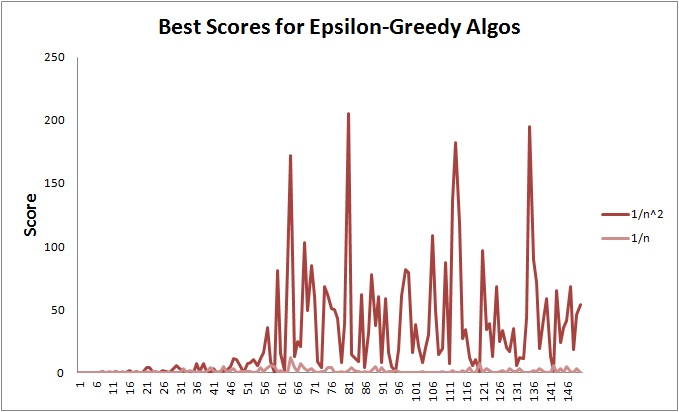
\includegraphics[width = 100mm] {score}
\]

\subsection{Optimizing Step 3}
After staring at our monkey making many, many jumps, we realized that step $iii)$ also wasn't ideal - instead of exploring, the monkey often would just jump where it wasn't supposed to. Instead of doing this, we decided to change the uniform choice to become the opposite choice that the $Q$-learning maximization would usually choose. This let the monkey perform actual exploration and not just choose randomly whenever $\epsilon$ was reached. Although we do not fully understand why this works, the hope is that this method is able to mitigate some of the issues of $Q$-learning where negative rewards to not propogate back well.

\subsection{Modified $\epsilon$-greedy Algorithm}
From the steps above, we reach our final algorithm:
\begin{enumerate}
\item[i)] Perform the Q-learning step, selecting the maximal $Q$ value for an action
\item[ii)] With probability $\epsilon \propto \frac{1}{n^2}$, where $n$ is the number of epochs that have passed:
\item[iii)] Select the step that has lower $Q$ value.
\end{enumerate}

\section{Parameter Tuning}
\subsection{State Space}
In our initial state space, we assumed that various parameters for symmetric. For example, we assumed the optimal threshold for leaving the screen was $50$ pixels on each side. After we tested this with the Q-Learning algorithm, we found more optimal values of parameters. Since the monkey tended to stay at the bottom more than the top (to have the option of coming back upwards), the height greater than 300 pixels actually performed better. To make sure that the result was significant, we ran the learner over several different learning cycles. We ended up seeing:
\[
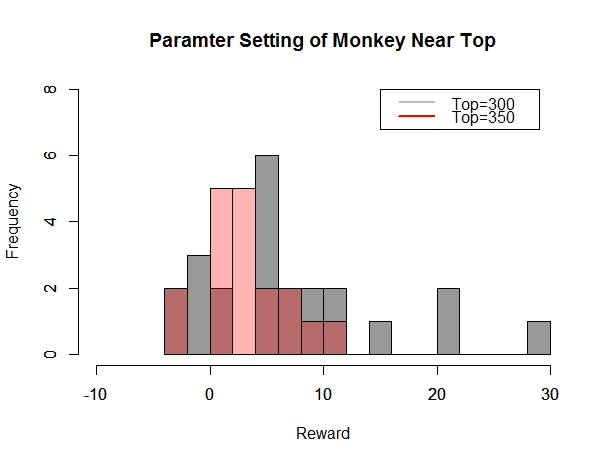
\includegraphics[width = 100mm] {top_param}
\]
Looking at the results, we can see that the change to a larger state meant that the variance increased a lot - there were cases when the monkey learned to do very well on average. We hypothesize that this is because the tree height usually stays below $300$, so this is helpful.

In addition, we found that having 10x10 blocks increased performance significantly, despite the increase in state space. We noticed this because the monkey was often hitting the tree by just a little bit. We hypothesized that if the monkey knew the state space just a little bit better, it would not miss as often by that small margin. This turned out to be correct:
\[
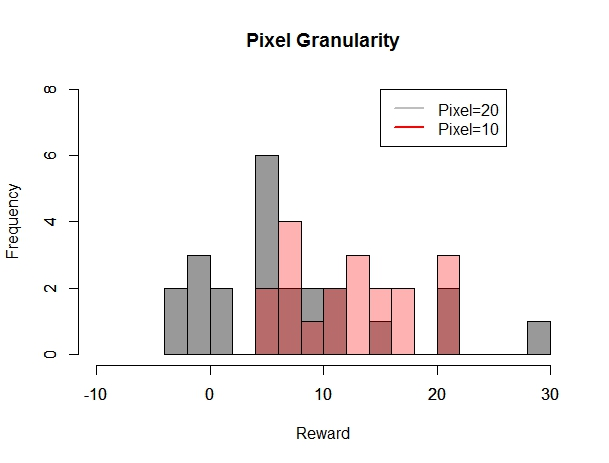
\includegraphics[width=100mm] {pixel_param}
\]
From this, we can see that having smaller blocks decreases variance drastically and increases the mean by a little bit. This decrease in variance can be explained by less monkeys missing trees by a little bit randomly.
\section{Conclusion}
We felt that we learned a lot about reinforcement learning in this practical. Although ideas such as Q-Learning are very nice on paper, in a murkier problem where the state space is not well defined, there can be a lot of different ways that people implement Q-Learning. In addition, although the problem seems very difficult at first glance, we saw how Q-Learning was able to capture a lot of the difficulty and leave us to tune its parameters such that the algorithm works. More specifically, for each of the portions of this practical, we felt like we took away:

\subsection{State Space}
Everything is feature selection. Feature selection is life.

\subsection{Q-Learning}
We realized while coding Q-Learning just how difficult realizing that there is a bug can be. After implementing Q-Learning the first time, we thought that we had gotten things correct and the rest of the practical would just be figuring out a good state space/improvements to the algorithm. It took us several hours to realize why our code was going so haywire was that our Q-Learning implementation actually had a bug in it.

\subsection{$\epsilon$-Greedy}
SwingyMonkey really defined the difference between theory and reality for us in terms of the $\epsilon$-Greedy extension. We covered in class that in theory, $\epsilon$-Greedy should only work with a variable on the order of $\frac{1}{n}$. However, realistically, because we could only run $100$ iterations and not $\infty$, we needed to use a more quickly vanishing $\epsilon$ to exploit the system enough by the time $100$ iterations ended.

As a result, we used an $\epsilon$ that doesn't satisfy any sort of property theoretically, one that decayed with $\frac{1}{n^2}$. However, because our monkey was able to exploit the game by epoch $100$, the monkey performed much better than the one with standard $\epsilon$-Greedy.
\end{document}